% This is LLNCS.DOC the documentation file of
% the LaTeX2e class from Springer-Verlag
% for Lecture Notes in Computer Science, version 2.4
\documentclass{llncs}
\usepackage{llncsdoc}
\usepackage{graphicx}
\usepackage{amssymb}
\usepackage{amsmath}
\usepackage{float}

\usepackage{caption}

\usepackage{enumitem}
\usepackage{booktabs}

\usepackage{multirow}

\usepackage{amsmath}

\usepackage{subcaption}
\captionsetup{compatibility=false}

\floatstyle{plaintop}
\restylefloat{table}

\DeclareMathOperator*{\argmin}{arg\,min} %argmin
%\usepackage[puttinydots,useemptybox]{braille}
%\usepackage{musixtex}
%
\begin{document}

\title{Clustering as a Tool of Reinforced Rejecting\\in Pattern Recognition Problem%\\with Rejecting Option
}
%\title{Rejecting Foreign Elements\\in Pattern Recognition Problem}
%\subtitle{Clustering as a Tool of Reinforced Rejecting}

\author{Jakub Ciecierski\inst{1}, Bartlomiej Dybisz\inst{1}, Agnieszka Jastrzebska\inst{1}\\\and Witold Pedrycz\inst{2,3}
}
\institute{$^1$Faculty of Mathematics and Information Science, Warsaw University of Technology\\
Plac Politechniki 1, 00-660 Warsaw, Poland\\
%\mailwh\\
%\url{http://www.mini.pw.edu.pl/~homenda}
$^2$Systems Research Institute, Polish Academy of Sciences\\ul. Newelska 6, 01-447 Warsaw, Poland\\
$^3$Department of Electrical \& Computer Engineering, University of Alberta\\Edmonton T6R 2G7 AB Canada
}

\authorrunning{J. Ciecierski, B. Dybisz, A. Jastrzebska, W. Pedrycz}
\titlerunning{Clustering as a Tool of Reinforced Rejecting}

\maketitle

\pagestyle{empty}  % no page numbers, no running headers

%-------------------------------------------------------------------
%-------------------------------------------------------------------
%-------------------------------------------------------------------
\begin{abstract}
Clustering is a common tool used in pattern recognition.
It aggregates similar elements from a given sample into one group, which is vital in the classification process.
In our study we consider a problem of discriminating foreign from
native elements.
Combined with geometrical approach and optimal grouping of native elements
we present a new way of constructing a recognizer.


\noindent\textbf{Keywords:} pattern recognition, cluster analysis, rejecting option, native and foreign elements
\end{abstract}


%-------------------------------------------------------------------
%-------------------------------------------------------------------
%-------------------------------------------------------------------
\section{Introduction}
  \label{Introduction}

The theoretical foundations for rejection were given by Chow \cite{Chow_1970}. He created the optimal rejection rule that optimizes a classification error. The solution was limited to binary classifiers and presented as a method for Bayes classifiers. Recognized elements are rejected when distance to a discrimination plane is
lower then a declared threshold. The optimal threshold is a~compromise between a number of misclassified elements and rejected correct results. The definition for a~multi{class issue was presented by Ha \cite{Ha_1997}. The Chow's rule is calculated for all pairs of classes separated by a discrimination plane.
There are also solutions for a~linear multi-classification task~\cite{Fumera2004}. However, most
of theoretical works is limited to the binary case \cite{Mascarilla2002}. A need of rejection option in practice of pattern recognition problem has been shown in many circumstances. Let us recall handwritten digits recognition \cite{BromleyDenker1993,Homenda_2015,RodrguezSanchezLlads} and optical music recognition, cf. \cite{Homenda_2005,Le1}

Motivation of this research is behind the need to process elements of the fixed set of classes as well as the ones not belonging to any class. In practice, given are characteristics of elements from fixed classes while no information about outside elements are known. Since we have no knowledge about elements not belonging to
any of the given classes, we can not use them in the process of recognizer construction. To distinguish between these two types of elements the following terms are used, cf.~\cite{Homenda_2015}: 
\begin{itemize}
  \item \textit{native} elements for elements of recognized classes and
  \item \textit{foreign} elements for ones not belonging to any given class.
\end{itemize}

In this study we perform cluster analysis in order to distinguish between native and foreign elements. The goal of such process is to obtain the most distinct clustering possible. The greater similarity between elements within a group and the greater the differences among other groups, the more distinct the clustering becomes. In this paper, we will try to find such $optimal$ clustering of native classes and observe effectiveness of such clustering in rejecting foreign elements. It is worth to underline that we do not consider classification of native elements. Interest is focused on separation native and foreign elements only.

Objectives of this study is to investigate clustering as a tool used for distinguishing between native and foreign elements. Invented methods are evaluated on synthetic data and then validated on real and semi-synthetic data.

The paper is structured as follows: in Section 2 concepts used in this work are introduced and then known topics of k-means algorithm, clustering evaluation and measures of rejecting quality are briefly described in order to make the paper self-contained. Further, in Section 3 previously described methods are tested and validated. Experiments are evaluated on synthetic data and then validated on real and semi-synthetic data. Finally, we conclude with final thoughts taken from our studies in Section 4.

%-------------------------------------------------------------------
%-------------------------------------------------------------------
%-------------------------------------------------------------------
\section{Methodology}
    \label{Preliminaries}

%-------------------------------------------------------------------
%-------------------------------------------------------------------
\subsection{Basic Concepts} 
  \label{basic_concepts}

Ordinary pattern recognition problem is an action of dividing a set of objects 
$\mathbf{S}=\{s_1, s_2\ldots,s_{\arrowvert\mathbf{S}\arrowvert}\}$ into subsets,
which include similar objects. Let us assume that $\mathbf{S}=\{S_1,S_2,\ldots,S_c\}$
such that $(\forall i \neq j)(S_i \cap S_j = \emptyset)$. Mapping $\sigma :\mathbf{S}\rightarrow \mathbf{C}$,
where $\mathbf{C}=\{1,2,\ldots,c\}$, constitutes a basic model for a task of splitting. 

% FEATURE VECTOR
Each object subjected to classification is defined by a vector of measurable characteristics, called features.
We assume that $\mathbf{X} = X_1 \times X_2 \times \ldots \times X_n = \mathbf{R}^{n}$
is the space of features.
A process of classification can be described by the two following mappings:
$\phi : \mathbf{S} \rightarrow \mathbf{X}$ and $\omega : \mathbf{X} \rightarrow \mathbf{C}$
The former one maps space of objects to space of features, and the latter one space of features to space of classes.
We can notice that $\sigma = \omega \circ \phi$, thus from now on we will refer to $\sigma$ as a classifier.


We will construct the rejector only on some part of considered space $\mathbf{S}$. 
Let $\mathbf{S} \supset \mathbf{L} = L_1 \cup L_2 \cup \ldots \cup L_{\vert\mathbf{C}\vert}$ 
such that $(\forall i \in \langle1,\vert\mathbf{C}\vert\rangle)(L_i \subset S_i)$. We call $\mathbf{L}$ a learning set.
Furthermore learning set is split into training set($\mathbf{Tr}$) and testing set($\mathbf{Ts}$) in the following fashion:
$\mathbf{L} = ( Tr_1 \cup Ts_1 ) \cup (Tr_2 \cup Ts_2 ) \cup \ldots \cup (Tr_{\vert C \vert} \cup Ts_{\vert\mathbf{C}\vert} )$
such that every class of the learning set is split into a~training set and a~testing set, namely: $(\forall i,j \in \langle1,\vert C \vert\rangle)(Tr_i \cup Ts_i = L_i \wedge Tr_i \cap Ts_j = \emptyset)$
and $\mathbf{Tr} = Tr_1 \cup Tr_2 \cup \ldots \cup Tr_{\vert\mathbf{C}\vert}$
along with $\mathbf{Ts} = Ts_1 \cup Ts_2 \cup \ldots \cup Ts_{\vert C\vert}$.
Finally each training set is grouped into clusters such that every element in that set belongs to exactly one group.

Let $\mathbf{Z} = Z_1 \cup Z_2 \cup \ldots \cup Z_{\vert C \vert}$ represent a~geometrical region in $\mathbf{R}^{n}$.
Each $Z_{i}$ is a geometrical figure which is assumed to enclose
all points of training set
$T_i$, where $i\in\langle1,\vert C \vert \rangle$.
Using this region we will determine if given feature vector 
represents a native or foreign element.

Since classification of native elements is not an aim of this study, an effort is focused on separation native elements from foreign ones. The following mapping is employed to formally describe the main objective of this study:
\begin{displaymath}
  \lambda : \mathbf{X} \rightarrow \mathbf{\bar{C}}\quad\textrm{such that}\quad(\forall x\in\mathbf{X})\;\;\lambda(x) = \left\{ 
  \begin{array}{ll}
    native & \textrm{if $x\in\mathbf{Z}$}\\
    foreign\qquad & \textrm{otherwise} %, i.e. $x\notin\mathbf{Z}$}
  \end{array} \right.
\end{displaymath}
In other words, if a~vector of features belongs to the region $\mathbf{Z}$, it is accounted as native one, otherwise it falls as foreign one.

Throughout this paper we use the word element to indicate examined object as well as its vector of features.
If the difference can not be distinguished from the context, we will refer to them explicitly.

%-------------------------------------------------------------------
%-------------------------------------------------------------------
\subsection{Geometry}
  \label{geometry}
  
To classify elements as either native of foreign we construct geometrical figures: ellipsoids and hyperrectangles. Each figure encloses some points belonging to the training set. Since these figures have been defined in great detail in our other paper, we recommend to refer to~\cite{rejecting_foreign_geo} for further reading on this matter.

%-------------------------------------------------------------------
%-------------------------------------------------------------------
\subsection{Evaluating}
  \label{evaluation}

Quality evaluation of classification with rejection requires non-standard measures. Intuitively, it is important to measure how exact rejection procedure is, i.e. how many foreign elements are (incorrectly) accepted and, vice versa, how many native elements are (incorrectly) rejected. Of course, measuring classification's quality understood as assigning native elements to proper classes is still of great importance, but does not affect our investigations, cf. \cite{Homenda_2015}.

For better understanding of how quality of classification with rejection should be measured we adopt parameters and quality measures used in signal detection theory. Since these parameters are widely utilized, we do not refer to original sources here. The following parameters were used in defining several measures outlining classification's quality. These parameters create so called confusion matrix, which is given in Table~\ref{tab:conf_matrix}. The parameters given in the matrix are numbers of elements of a~testing set which have the following meaning:

\vspace{-9pt}
\begin{table}[!t]
\vspace{-3pt}
\caption{Confusion matrix for rejecting in pattern recognition problem}
\centering
\begin{tabular}{|c|c|c|}
\hline
  & & \vspace{-6pt}\\
  & \hspace{12pt}Classification to the class\hspace{12pt} & \hspace{3pt}Exclusion from the class\hspace{3pt} \\
  & & \vspace{-6pt}\\
\hline 
  & & \vspace{-6pt}\\
  The class & True Positives (TP) & False Negatives (FN) \\
  & & \vspace{-6pt}\\
\hline
  & & \vspace{-6pt}\\
  \hspace{3pt}Not the class\hspace{3pt} & False Positives (FP) &  True Negatives (TN)\\[5pt]
\hline
\end{tabular}
\vspace{-9pt}
\label{tab:conf_matrix}
\end{table}
\begin{itemize}
  \item $TP$ - the number of elements of the considered class correctly classified to the given class,
  \item $FN$ - the number of elements of the considered class incorrectly excluded from the given class,  
  \item $FP$ - the number of elements of other classes incorrectly classified to the given class,  
  \item $TN$ - the number of elements of other classes correctly excluded from the given class.  
\end{itemize}  

In this study, original pattern recognition problem is a multi-class problem. However, from rejecting point of view, important is whether a native element is classified to any native class, even incorrect native class. Therefore, the question if native elements is classified to the correct or any other native class is not considered. Hence, a multi class pattern recognition with rejection is turned to two-classes problem. Finally, the following measures were used assess the quality of the classifier:
%\begin{flalign}
\begin{eqnarray}
  \textnormal{Accuracy}    & = &   \displaystyle\frac{\textnormal{TP+TN}}{\textnormal{TP+FN+FP+TN}}\nonumber\\
  \textnormal{Sensitivity} &\;=\;& \displaystyle\frac{\textnormal{TP}}{\textnormal{TP+FN}}\nonumber\\
  \textnormal{Precision}   & = &   \displaystyle\frac{\textnormal{TP}}{\textnormal{TP+FP}}\nonumber\\
  \textnormal{F--measure}  &\;=\;& 2\cdot\frac{\mbox{Precision}\cdot\mbox{Sensitivity}}{\mbox{Precision}+\mbox{Sensitivity}}
\end{eqnarray}

%-------------------------------------------------------------------
%-------------------------------------------------------------------
\subsection{Cluster Analysis}
  \label{clustering}
As stated previously the training set of each class is split into clusters. In other words, the space of a given class is now defined by geometrical figures constructed on these clusters. An important objective in our study is finding an optimal number of clusters. In order to accomplish that we perform cluster evaluation described in this section.

\vspace{-6pt}
%-------------------------------------------------------------------
\subsubsection{k-means}
  \label{k_means}

The well known k-means algorithm is employed for clustering. Let's assume that a~data set $X$ of size $n$ is going to be partitioned into $k$ number of clusters and each element $x_{j}\in X$ is assigned a~cluster. In order to do that, we find cluster centers $\mu_{i}, i=1,\ldots,k$ that minimize the distance from the elements from data set. Formally k-means solves the following optimization problem:
\begin{equation}
  \argmin_{C}\sum_{i=1}^{k}\sum_{x\in C_{i}} d(x,\mu_{i})
\end{equation}
where $C_{i}$ is the set of elements that correspond to $i$-th cluster and $d(x,\mu_{i})$ is a~chosen distance measure between element $x$ and the cluster center $\mu_{i}$. At the first stage of the algorithm k centers $\mu_{i}$ are selected. Then each element is assigned to the closest cluster. The centers are updated with the mean of all points belonging to the corresponding cluster
\begin{equation}
  \mu_{i} = \frac{1}{|C_{i}|} \sum_{x\in C_{i}} x
\end{equation}

This process is repeated until convergence. It is worth mentioning that k-means might not find the best possible 
configuration.

%-------------------------------------------------------------------
%-------------------------------------------------------------------
\subsubsection{Prediction Strength}
  \label{cluster_evaluation}

Evaluation of clustering is performed using a method called {\it prediction strength}. Dataset $X$, for which clustering is performed, is split into training set $X_{tr}$ and testing set $X_{te}$. The split is random. Both sets are then subjected to clustering. Let us denote the clustering operation by $C(X,k)$, where $X$ is the data set and $k$ the number of clusters. In our study we use k-means clustering algorithm. For each pair of elements belonging to the same testing cluster, we determine if they belong to the same cluster in training set, based on the distance from its center. To accomplish that we will define a $|X_{te}|\times|X_{te}|$ matrix 
$D[C(X_{tr},k), X_{te}]$ in which each entry is called a co-membership, namely 
$D[C(X_{tr},k), X_{te}]_{ii'} = 1$ if elements $i$ and $i'$ belong to the same training cluster - 
computed from set $X_{tr}$, 0 otherwise.
Let $T_{1}, T_{2}, \ldots, T_{k}$ denote set of indices of test observations in consecutive 
test clusters with respective sizes $m_{1}, m_{2}, \ldots, m_{k}$.
We define prediction strength by

\begin{equation}
  ps(k) = \min_{1 \leq j \leq k} \frac{1}{m_{j}(m_{j}-1)} 
  \sum_{i,i'\in T_{j},i\ne i'} D[C(X_{tr},k), X_{te}]_{ii'}
\end{equation}

Finally, to reduce influence of randomness, the average of prediction strength is taken for several data splits into training and testing sets. The optimal number of clusters is such $k>1$ that maximizes $ps(k)$. For further information refer to~\cite{pred_strength}.



%-------------------------------------------------------------------
%-------------------------------------------------------------------
%-------------------------------------------------------------------
\section{Experiment}
    \label{Experiment}

In this study experiments are performed on synthetic, semi-synthetic and real datasets. The former one were used to evaluate correctness of prediction strength method. The real and semi-synthetic datasets were used to check the effectiveness of our rejector. In this case the datasets where subjected to k-means clustering. Then, based on these clusters, ellipsoids and hyperrectangles enclosing clusters were constructed, cf.~\cite{rejecting_foreign_geo}. Finally, results for different number of clusters are compared. It is worth to underline again that classification of native elements to correct classes is not considered in this study, instead separation of native elements from foreign ones is investigated.

%-------------------------------------------------------------------
%-------------------------------------------------------------------
\subsection{Synthetic Data}

%-------------------------------------------------------------------
\subsubsection{Datasets}

Carefully constructed synthetic data were used to check correctness of prediction strength. We created ten native classes having observations in 24-dimensional space. For each class $k'$ centers were generated.
Then 1000 observations were spread around these centers using normal probability distribution to obtain a class having $k'$ clouds. Figure~\ref{fig:plot_clouds} shows the idea of data generation in a 3-dimensional space.
In the experiment we created classes with $k' = 2,3,4$ and $5$ clouds and computed their prediction strength for $k=1,2,\ldots,7$.
\begin{figure}[!h]
\begin{subfigure}[b]{0.33\linewidth}
\centering
  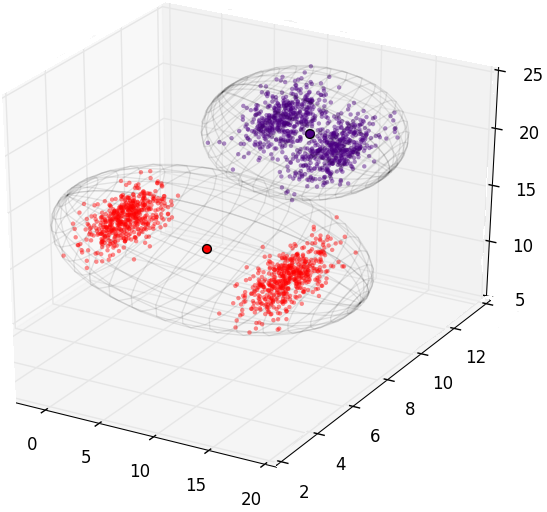
\includegraphics[width=40mm]{_Figures/plot/k1_small}
  \caption{one cluster}
   \label{fig:k1}
\end{subfigure}%
\begin{subfigure}[b]{0.33\linewidth}
\centering
  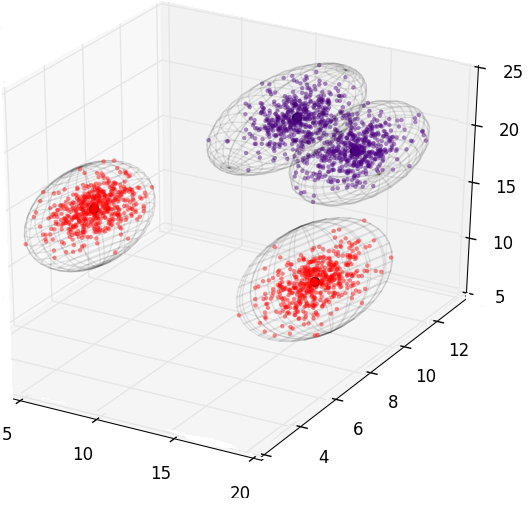
\includegraphics[width=40mm]{_Figures/plot/k2_small}
  \caption{two clusters}
  \label{fig:k2}
\end{subfigure}%
\begin{subfigure}[b]{0.33\linewidth}
\centering
  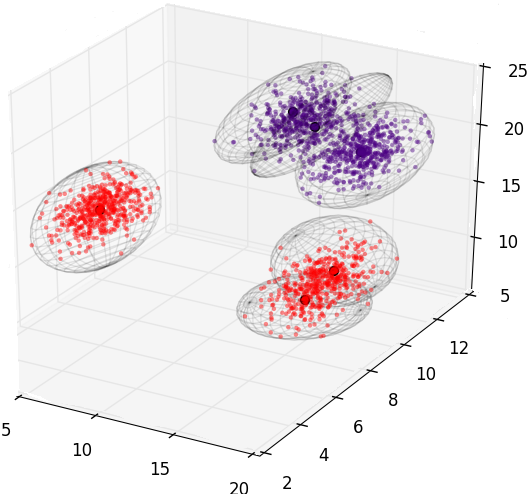
\includegraphics[width=40mm]{_Figures/plot/k3_small}
  \caption{three clusters}
  \label{fig:k3}
\end{subfigure}%
\caption{Illustration of synthetic native data. Two classes are colored in red and indigo. Each class has $k' = 2$ $clouds$ of elements. Clustering is into one, two and three clusters, respectively.}
  \label{fig:plot_clouds}
\vspace{-12pt}
\end{figure}

% Foreign
Two foreign sets were generated. A homogeneous set of foreign elements was created by applying uniform distribution in the same intervals of every dimension as used for generating native classes. A non-homogeneous set was obtained by locating centers between pairs of native classes and generating cloud of elements around such centers.
 

%-------------------------------------------------------------------
\subsubsection{Results}

Table~\ref{tab:ps_synth} shows the results of prediction strength. For example when $k'=2$, the predicted number of clusters is $k=2$. In general we see that optimal $k$ value is equal to $k'$, i.e. $ps(k')=k$. We can also notice that once the true number of clusters has been found, the value of prediction strength decreases for finer clustering.

In Table~\ref{tab:confusion_matrix_synthetic1} confusion matrix for rejecting foreign elements is presented. The synthetic learning set of elements was generated with $k'=3$ {\it clouds} for each class. Hence, prediction strength clustering measure should favor clustering to $k=3$ clusters.

As we can see, rejection quality is slightly better for the homogeneous foreign set than for non-homogeneous one for both types of figures, what justifies qualitative compatibility of used figures.

Let us focus our attention on hyperrectangles for non-homogeneous set. We notice that in the case of two clusters, the count of rejected foreign elements (TN) was rather small. In this case, the hyperrectangles took a lot of space between native clouds, which was occupied by foreign elements, but not by native ones. Recalling that the foreign elements were generated between native classes, we can conclude that many of such elements were included in such figures.

\begin{table}[!t]
\centering
\caption{Prediction strength for different number of clouds (k') and clusters (k)}
\setlength{\tabcolsep}{10pt}
\renewcommand{\arraystretch}{1.3}
\begin{tabular}{|r||c|c|c|c|}
\hline
$ps(k)$ & \multicolumn{4}{c|}{ $k'$ } \\
\hline
 $k$ & $2$ & $3$ & $4$ & $5$\\
\hline
\hline
2  & $1.00$ & $0.60$ & $1.00$ & $0.95$  \\
3  & $0.51$ & $1.00$ & $0.80$ & $0.53$  \\
4  & $0.50$ & $0.52$ & $1.00$ & $0.95$  \\
5  & $0.34$ & $0.50$ & $0.51$ & $1.00$  \\
6  & $0.33$ & $0.48$ & $0.50$ & $0.53$  \\
7  & $0.24$ & $0.34$ & $0.49$ & $0.50$  \\
   \hline
\end{tabular}
\label{tab:ps_synth}
\end{table}

\begin{table}[!t]
\caption{Confusion matrices for synthetic foreign sets. Columns correspond to geometric figures, rows - to number of clusters. Row labelled $Optimal$ represents grouping with optimal number of clusters.}
\label{tab:confusion_matrix_synthetic1}
\centering
\setlength{\tabcolsep}{6pt}
\renewcommand{\arraystretch}{1.1}
\begin{tabular}{|r||rr||rr||rr||rr|}
\hline
  & \multicolumn{8}{c|}{ rejector based on } \\
\hline
data set & \multicolumn{4}{c||}{ homogeneous } & \multicolumn{4}{c|}{ non-homogeneous} \\
\hline
figure &  \multicolumn{2}{c||}{hyperrect} & \multicolumn{2}{c||}{ellipsoids} & \multicolumn{2}{c||}{hyperrect} & \multicolumn{2}{c|}{ellipsoids} \\
\hline
\hline
confusion & \multicolumn{2}{c||}{\;TP$\qquad$FN} & \multicolumn{2}{c||}{\;TP$\qquad$FN} & \multicolumn{2}{c||}{\;TP$\qquad$FN} & \multicolumn{2}{c|}{\;TP$\qquad$FN} \\
matrix & \multicolumn{2}{c||}{\;FP$\qquad$TN} & \multicolumn{2}{c||}{\;FP$\qquad$TN} & \multicolumn{2}{c||}{\;FP$\qquad$TN} & \multicolumn{2}{c|}{\;FP$\qquad$TN} \\
\hline
\hline
	& $93.67$ & $6.33$  
	& $82.75$ & $17.25$  
	& $93.67$ & $6.33$   
	& $82.75$ & $17.25$  \\
2 
	& $1.10$  & $98.90$ 
	& $0.01$  & $99.99$ 
	& $36.40$ & $63.60$ 
	& $4.52$  & $95.48$ \\
\hline
     & $90.52$  & $9.48$  
     & $75.24$  & $24.76$ 
     & $90.52$  & $9.48$ 
     & $75.24$  & $24.76$  \\
 3 (Optimal) 
	 & $0.22$   & $99.78$ 
	 & $0.02$   & $99.98$ 
	 & $16.06$  & $83.94$  
	 & $1.82$   & $98.18$ \\
\hline
     & $89.40$  & $10.60$ 
     & $69.60$  & $30.40$  
     & $89.40$  & $10.60$   
     & $69.60$  & $30.40$ \\
 4 
	 & $0.19$   & $99.81$ 
	 & $0.01$   & $99.99$ 
	 & $14.03$  & $85.97$  
	 & $1.50$   & $98.50$ \\
\hline
     & $88.19$  & $11.81$  
     & $64.62$  & $35.38$  
     & $88.19$  & $11.81$  
     & $64.62$  & $35.38$ \\
 5 
	& $0.17$   & $99.83$
	& $0.01$   & $99.99$ 
	& $12.84$  & $87.16$  
	& $0.89$   & $99.11$ \\
   \hline
\end{tabular}
\vspace{-6pt}
\end{table}

%-------------------------------------------------------------------
\subsubsection{Summary}

Empirical verification of invented methods was done as follows:
\begin{itemize}
  \item prediction strength measure was employed in finding optimal clustering of training sets of native classes,
  \item training sets of native classes were split to 2, 3, 4 and 5 clusters with k-means algorithm employed,
  \item for every split constructed were minimal volume hyperrectangles and ellipsoids enclosing clusters,
  \item rejection quality was evaluated for testing sets.
\end{itemize} 
Table~\ref{tab:rejection_results_synthetic} summarizes rejection results for testing set of synthetic data. 
As it is shown, rejecting quality depends on clustering optimality in the sense that it provides a trade-off between different measures of rejecting quality. The optimality of clustering did not play a significant role in the case of uniformly distributed foreign elements. For instance, there is a~balance between acceptance of native elements and rejecting foreign ones, cf. F-measure. We can see that for hyperrectangles, F-measure peaks up slightly the optimal number of clusters. In other words we are capable of rejecting fair amount of foreign elements while having high sensitivity to classifying native ones.

Each time the number clusters is increase, sensitivity is decreased. In case of the ellipsoids the drop is stronger. By adding more clusters we essentially lower the space that native classes cover, thus the probability of classifying native elements drops with it. With the knowledge of how the recognizer behaves in various test cases, we move to validate our methods on real data.

\begin{table}[!t]
\centering
\caption{Summary of rejector quality for synthetic data sets. Abbreviation h-r stands for hyperrectangle, ell - for ellipsoid}
\label{tab:rejection_results_synthetic}
\setlength{\tabcolsep}{5pt}
\renewcommand{\arraystretch}{1.1}
\begin{tabular}{|r||c|c||c|c||c|c||c|c||c|c|}
\hline
data set 
  	& \multicolumn{8}{c|}{homogeneous} \\
\hline
clusters 
  	& \multicolumn{2}{c||}{2} 
  	& \multicolumn{2}{c||}{3 (Optimal)} 
  	& \multicolumn{2}{c||}{4} 
  	& \multicolumn{2}{c|}{5}\\
\hline
geometry 
	& h-r & ell & h-r & ell & h-r & ell & h-r & ell \\
\hline
\hline
Accuracy   
	& $0.96$ & $0.91$ 
	& $0.95$ & $0.88$ 
	& $0.95$ & $0.85$ 
	& $0.94$ & $0.82$  \\
Sensitivity 
	& $0.94$ & $0.83$ 
	& $0.91$ & $0.75$ 
	& $0.89$ & $0.70$ 
	& $0.88$ & $0.65$  \\
Precision  
	& $0.99$ & $0.99$ 
	& $0.99$ & $0.99$ 
	& $0.99$ & $0.99$ 
	& $0.99$ & $0.99$  \\
F-measure   
	& $0.96$ & $0.91$ 
	& $0.95$ & $0.85$ 
	& $0.94$ & $0.82$ 
	& $0.94$ & $0.79$  \\
   \hline
\end{tabular}

\vspace{10pt}

\centering
\setlength{\tabcolsep}{5pt}
\renewcommand{\arraystretch}{1.1}
\begin{tabular}{|r||c|c||c|c||c|c||c|c||c|c|}
\hline
data set 
  	& \multicolumn{8}{c|}{non-homogeneous} \\
\hline
clusters 
  	& \multicolumn{2}{c||}{2} 
  	& \multicolumn{2}{c||}{3 (Optimal)} 
  	& \multicolumn{2}{c||}{4} 
  	& \multicolumn{2}{c|}{5}\\
\hline
geometry 
	& h-r & ell & h-r & ell & h-r & ell & h-r & ell \\
\hline
\hline
Accuracy   
	& $0.79$ & $0.89$ 
	& $0.87$ & $0.87$ 
	& $0.88$ & $0.84$ 
	& $0.88$ & $0.82$  \\
Sensitivity 
	& $0.94$ & $0.83$ 
	& $0.91$ & $0.75$ 
	& $0.89$ & $0.70$ 
	& $0.88$ & $0.65$  \\
Precision  
	& $0.72$ & $0.95$ 
	& $0.85$ & $0.98$ 
	& $0.86$ & $0.98$ 
	& $0.87$ & $0.99$  \\
F-measure   
	& $0.81$ & $0.88$ 
	& $0.88$ & $0.85$ 
	& $0.87$ & $0.81$ 
	& $0.87$ & $0.78$  \\
   \hline
\end{tabular}
\end{table}

%-------------------------------------------------------------------
%-------------------------------------------------------------------
\subsection{Real and Semi-Synthetic Data}

%-------------------------------------------------------------------
\subsubsection{Datasets}

The datasets were constructed based on the~MNIST database of handwritten digits \cite{LeCunCortesBurges}. 
In this experiment we operated on two sets of classes: native (real data) and foreign (semi-synthetic).
Both native and foreign sets consisted of 10000 elements. Each element was described by a~vector of 24 features.
In native set each element belonged to one of 10 classes of handwritten digits. Figure~\ref{fig:digits_native} shows samples of native elements.

\begin{figure}[!t]
  \centering
  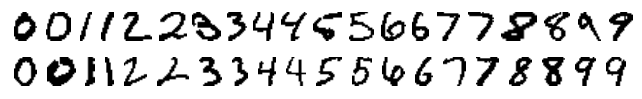
\includegraphics[width=0.67\columnwidth]{_Figures/native}
  \caption{Samples of elements from native classes.}
  \label{fig:digits_native}
  \vspace{6pt}
  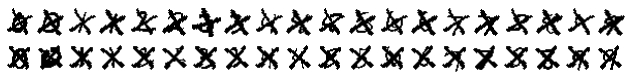
\includegraphics[width=0.67\columnwidth]{_Figures/crossedout.png}
  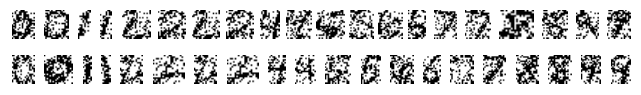
\includegraphics[width=0.67\columnwidth]{_Figures/xor.png}
  \caption{Samples of foreign elements.}
  \label{fig:digits_foreign}
  \vspace{-12pt}
\end{figure}

Two different foreign sets were constructed by applying a certain distortion to native elements. In set $A$ elements were constructed by crossing out native ones. Set $B$ included native elements distorted by a random salt-and-pepper noise XOR-ed with source pixels. Samples of foreign elements are displayed in Figure~\ref{fig:digits_foreign}. Notice that foreign elements are treated as a whole without distinguishing original classes, from which they were created.

Native classes were split into learning and testing sets. Each class was subjected to k-means clustering based on its learning set. Then the minimal volume hyperrectangles and ellipsoids enclosing every cluster were constructed.

\vspace{-6pt}
%-------------------------------------------------------------------
\subsubsection{Results}
% Prediction strength
Table~\ref{tab:ps_native} presents results for cluster evaluation for all native classes (each class represents a digit). In this case, prediction strength indicates that a favourable clustering is based on small number of clusters. The optimal number of clusters for each class varies from two to three.
This suggests that there are similarities between native classes, to be precise between features vectors describing native classes, and we are able to detect and join similar native classes.

% Intro to results
Table~\ref{tab:confusion_matrix_real} is a confusion matrix for a two class problem for native contra foreign elements. It presents an evaluation of recognizers' quality. Compared are models based on two geometric figures: hyperrectangle and ellipsoid. Each row gathers information about results concerning different number of clusters into which the native classes were grouped.

% General notes
Let us take into consideration the construction method of geometric figures forming analysed models. Each created figure has a minimal possible volume necessary to enclose all points of a given cluster. Hyperrectangles embrace larger subset of the space than ellipsoids. As a result, hyperrectangles achieve excellent results for correct classification of native elements (TP and FN). The downside of hyperrectangles-based models is that the superior recognition of native elements is at cost of a lowered quality of foreign elements rejection. 

In contrast, ellipsoids-based models enclosing the same set of points, have considerably smaller volume. Hence, in this case rejecting foreign elements becomes  easier, while classifying native ones proves to be a difficult task.


\begin{table}[!t]
\caption{Results of prediction strength for different native classes and different number of clusters.} 
\vspace{-2pt}
\label{tab:ps_native}
\centering
\setlength{\tabcolsep}{8pt}
\renewcommand{\arraystretch}{1.3}
\begin{tabular}{|r||c|c|c|c|c|c|c|c|c|c|}
\hline
  & \multicolumn{10}{c|}{ Class } \\
\hline
  k & $0$ & $1$ & $2$ & $3$ & $4$ & $5$ & $6$ & $7$ & $8$ & $9$ \\
\hline
\hline
2  & $0.92$ & $0.89$ & $0.53$ & $0.96$ & $0.86$ & $0.95$ & $0.83$ & $0.72$ & $0.74$ & $0.94$  \\
3  & $0.86$ & $0.93$ & $0.85$ & $0.55$ & $0.86$ & $0.78$ & $0.94$ & $0.52$ & $0.75$ & $0.72$  \\
4  & $0.71$ & $0.80$ & $0.53$ & $0.58$ & $0.77$ & $0.82$ & $0.73$ & $0.42$ & $0.71$ & $0.61$  \\
5  & $0.55$ & $0.50$ & $0.50$ & $0.40$ & $0.77$ & $0.63$ & $0.48$ & $0.61$ & $0.52$ & $0.71$  \\
6  & $0.43$ & $0.49$ & $0.39$ & $0.53$ & $0.42$ & $0.39$ & $0.43$ & $0.40$ & $0.38$ & $0.68$  \\
7  & $0.40$ & $0.43$ & $0.47$ & $0.44$ & $0.45$ & $0.43$ & $0.47$ & $0.33$ & $0.38$ & $0.46$  \\
   \hline
\end{tabular}
\end{table}

\begin{table}[!t]
\caption{Confusion matrix of real and semi-synthetic data. Columns correspond to figures, rows - to numbers of clusters. Row labelled $Optimal$ represents allocation of each class into its optimal number of clusters.}
\label{tab:confusion_matrix_real}
\centering
\setlength{\tabcolsep}{6pt}
\renewcommand{\arraystretch}{1.1}
\begin{tabular}{|r||rr||rr||rr||rr|}
\hline
  & \multicolumn{8}{c|}{rejector based on} \\
\hline
foreigns & \multicolumn{4}{c||}{ A } & \multicolumn{4}{c|}{ B} \\
\hline
geometry &  \multicolumn{2}{c||}{hyperrect} & \multicolumn{2}{c||}{ellipsoids} & \multicolumn{2}{c||}{hyperrect} & \multicolumn{2}{c|}{ellipsoids} \\
\hline
\hline
confusion & \multicolumn{2}{c||}{\;TP$\qquad$FN} & \multicolumn{2}{c||}{\;TP$\qquad$FN} & \multicolumn{2}{c||}{\;TP$\qquad$FN} & \multicolumn{2}{c|}{\;TP$\qquad$FN} \\
matrix & \multicolumn{2}{c||}{\;FP$\qquad$TN} & \multicolumn{2}{c||}{\;FP$\qquad$TN} & \multicolumn{2}{c||}{\;FP$\qquad$TN} & \multicolumn{2}{c|}{\;FP$\qquad$TN} \\
\hline
\hline
	     & $95.41$ & $4.59$  & $68.25$ & $31.75$  &   $96.67$ & $3.33$   & $70.48$ & $29.52$  \\
Optimal & $34.58$   & $65.42$ & $0.30$   & $99.70$ &   $60.46$  & $39.54$ & $0.83$  & $99.17$ \\
\hline
     & $96.99$  & $3.01$  & $75.01$  & $24.99$  &   $96.57$  & $3.43$  & $74.52$  & $25.48$  \\
 2 & $41.86$   & $58.14$ & $0.63$   & $99.37$ &   $60.52$  & $39.48$ & $0.64$  & $99.36$ \\
\hline
     & $93.82$  & $6.18$  &  $63.80$  & $36.20$  &  $94.22$  & $5.78$  & $64.89$  & $35.11$  \\
 3 & $30.71$   & $69.29$ & $0.19$   & $99.81$ &  $58.96$  & $41.04$  & $1.80$   & $98.20$ \\
\hline
     & $92.61$  & $7.39$  & $53.89$  & $46.11$  & $90.42$  & $9.58$   & $54.07$  & $45.93$ \\
 4 & $23.98$   & $76.02$ & $0.04$   & $99.96$ &  $46.86$  & $53.14$  & $1.25$   & $98.75$ \\
\hline
     & $87.61$  & $12.39$  & $46.27$  & $53.73$  &  $89.12$  & $10.88$  & $45.26$  & $54.74$ \\
 5 & $17.35$   & $82.65$ & $0.03$   & $99.97$ &  $41.17$  & $58.83$  & $0.05$   & $99.95$ \\
   \hline
\end{tabular}
\vspace{-6pt}
\end{table}

% Notice about error in calculations
Let us point out a small difference in parameters associated with classification of native elements (TP and FN) in the two different foreign sets within the same geometric figure. This small error is caused by random split into learning and testing sets.

% Compare two sets
Ellipsoids proved to be equally effective in both foreign sets, rejecting more than $96\%$ of elements across the board. In contrast, there is a discrepancy between two foreign sets for hyperrectangles-based models. Set B, which was created by crossing out native elements, turned out to be more difficult to reject.


% Clustering
Finally, let us analyse differences in quality of recognition for models based on various clustering configurations. We have observed that when the number of clusters gets increased, the space that defines a single class usually shrinks. This is manifested with a decrease of TP and an increase of TN values for increasing number of clusters. As it has been pointed out before, experiments indicate that the optimal number of clusters is either two of three. This conclusion is supported by the results presented in the confusion matrix.

\vspace{-6pt}
%-------------------------------------------------------------------
\subsubsection{Summary}
% Classifier assesment
Table~\ref{tab:rejection_results_real} presents measures summarizing the quality of the classifier for each foreign set.

Sensitivity informs about the quality of native elements classification. Table~\ref{tab:rejection_results_real} shows that sensitivity of ellipsoids tends to decrease quite fast as the number of clusters grows. Let us recall, that we operated on the same native set. Hence, the sensitivity in the two tables is approximately the same.

Application of optimal clustering was not beneficial for ellipsoids-based model. In this case, precision was already at its peak with two clusters. When more clusters are added, a chance for correct classification of native elements gets lowered. Hence, we may obtain lower sensitivity and accuracy values at the same time.

When it comes to hyperrectangles, the f-measure and accuracy increased slightly. We have observed that hyperrectangles are less compact figures and they tend to overlap. In other words, adding clusters gave more space to reject foreign elements while maintaining the probability to accept native elements reasonable high.

\begin{table}[!t]
\caption{Summary of rejector quality for semisynthetic foreign elements. Abbreviation h-r stands for hyperrectangle, while ell - for ellipsoid.}
\label{tab:rejection_results_real}
\centering
\setlength{\tabcolsep}{5pt}
\renewcommand{\arraystretch}{1.1}
\begin{tabular}{|r||c|c||c|c||c|c||c|c||c|c|}
\hline
data set 
  	& \multicolumn{10}{c|}{Set A of semisynthetic foreign elements} \\
\hline
clusters 
	& \multicolumn{2}{c||}{Optimal} 
  	& \multicolumn{2}{c||}{2} 
  	& \multicolumn{2}{c||}{3} 
  	& \multicolumn{2}{c||}{4} 
  	& \multicolumn{2}{c|}{5}\\
\hline
geometry 
	& h-r & ell & h-r & ell & h-r & ell & h-r & ell & h-r & ell\\
\hline
\hline
Accuracy   
	& $0.80$ & $0.84$ & $0.78$ & $0.87$ & $0.82$ 
	& $0.82$ & $0.84$ & $0.77$ & $0.85$ & $0.73$ \\
Sensitivity 
	& $0.95$ & $0.68$ & $0.97$ & $0.75$ & $0.94$ 
	& $0.64$ & $0.93$ & $0.54$ & $0.88$ & $0.46$ \\
Precision  
	& $0.73$ & $0.99$ & $0.69$ & $0.99$ & $0.75$ 
	& $0.99$ & $0.79$ & $0.99$ & $0.83$ & $0.99$ \\
F-measure   
	& $0.83$ & $0.81$ & $0.81$ & $0.85$ & $0.84$ 
	& $0.78$ & $0.86$ & $0.70$ & $0.85$ & $0.63$ \\
   \hline
\end{tabular}

\vspace{6pt}

\centering
\setlength{\tabcolsep}{5pt} % TODO 
\renewcommand{\arraystretch}{1.1}
\begin{tabular}{|r||c|c||c|c||c|c||c|c||c|c|}
\hline
data set 
  	& \multicolumn{10}{c|}{Set B of semisynthetic foreign elements} \\
\hline
  clusters 
  	& \multicolumn{2}{c||}{Optimal} 
  	& \multicolumn{2}{c||}{2} 
  	& \multicolumn{2}{c||}{3} 
  	& \multicolumn{2}{c||}{4}  
  	& \multicolumn{2}{c|}{5}\\
\hline
  geometry & h-r & ell & h-r & ell & h-r & ell & h-r & ell & h-r & ell\\
\hline
\hline
Accuracy    
	& $0.68$ & $0.85$ & $0.68$ & $0.87$ & $0.68$ 
	& $0.82$ & $0.72$ & $0.76$ & $0.74$ & $0.73$ \\
Sensitivity 
	& $0.97$ & $0.70$ & $0.97$ & $0.75$ & $0.94$ 
	& $0.65$ & $0.90$ & $0.54$ & $0.89$ & $0.45$ \\
Precision   
	& $0.62$ & $0.99$ & $0.61$ & $0.99$ & $0.62$ 
	& $0.97$ & $0.66$ & $0.98$ & $0.68$ & $0.99$ \\
F-measure   
	& $0.75$ & $0.82$ & $0.75$ & $0.85$ & $0.74$ 
	& $0.78$ & $0.76$ & $0.69$ & $0.77$ & $0.62$ \\
   \hline
\end{tabular}
\end{table}

%-------------------------------------------------------------------
%-------------------------------------------------------------------
%-------------------------------------------------------------------
\vspace{-6pt}
\section{Conclusions}
\vspace{-6pt}

Carried experiments aimed at constructing a model for distinguishing native and foreign elements. In this study all native elements are treated as one big class. Hyperrrectangles and ellipsoids are considered as classification vehicles. Elements embraced by them are accounted as native. Remaining elements are rejected and treated as foreign. A series of experiments has been executed, focusing on a broad suite of datasets, from synthetic to real, for different numbers of different figures used for classification. Quality of trained models both with respect to recognition of native elements and to rejection of foreign ones is analysed.

Experiments show that hyperrectangles are an effective tool in identification of native elements. However, models based on ellipsoids provide higher precision of rejecting foreign elements. 

A series of tests has been conducted to check if a knowledge about optimal number of clusters in the natives' dataset could improve rejection of foreign elements. The optimal number of clusters has been detected and applied in the model design phase in hope to obtain best possible results. This strategy provided superior rejection of foreign elements, but at the same time it hindered accuracy of native elements' classification.

%In future, we plan to develop further this geometrical-based approach to foreign elements rejection. 

%If one would consider clustering set of $n$ native elements into $n$ groups, it would suddenly become nearly impossible to obtain any reasonable sensitivity.


%-------------------------------------------------------------------
%-------------------------------------------------------------------
%-------------------------------------------------------------------
\vspace{-6pt}
\section*{Acknowledgement}
\vspace{-6pt}
The research is supported by the National Science Center,\\grant No 2012/07/B/ST6/01501, decision no UMO�2012/07/B/ST6/01501.
\vspace{-6pt}
\begin{thebibliography}{19}
\vspace{-6pt}
\bibitem{BromleyDenker1993}
J. Bromley, J.S. Denker, Improving rejection performance on handwritten digits by training with rubbish. Neural Computing, 5, 367-370, 1993

\bibitem{Chow_1970}
Chow, C., On optimum recognition error and reject tradeoff, IEEE Transactions on Information Theory, 16(1), 41-46, 1970

\bibitem{rejecting_foreign_geo}
Ciecierski J., Dybisz B., Jastrzebska A., Pedrycz W., Rejecting Foreign Elements in Pattern Recognition Problem: A Geometrical Approach, submitted to CISIM 2015

\bibitem{Fumera2004}
Fumera, G., Roli, F.: Analysis of error-reject trade-off in linearly combined multiple classifiers, Pattern Recognition, 37, 1245-1265, 2004

\bibitem{Ha_1997}
Ha, T.: Optimum Tradeoff between Class-selective Rejection Error and Average Number of Classes, Engineering Applications of Artificial Intelligence, 10(6), 525-529, 1997

\bibitem{Homenda_2015}
Homenda W., Jastrzebska A. and Pedrycz W., Rejecting Foreign Elements in Pattern Recognition Problem: Reinforced Training of Rejection Level, Proc. of the 7th International Conference on Agents and Artificial Intelligence, pp. 90-99, 2015

\bibitem{Homenda_2005}
Homenda W., Optical music recognition: The case study of pattern recognition, in: Computer Recognition Systems, Advances in Soft Computing, Kurzynski, M; Puchala, E; Wozniak, M; et al. (Eds), 835-842, 2005

\bibitem{Le1}
Homenda W., Lesinski W., Optical Music Recognition: Case of Pattern recognition with Undesirable and Garbage Symbols, in: Image Processing and Communications Challenges, Choras R. et al (Eds.), 120-127, 2009

\bibitem{LeCunCortesBurges}
LeCun, Y., Cortes, C., and Burges, C. (1996). The MNIST database of handwritten digits. In http://yann.lecun.com/exdb/mnist/.

\bibitem{Mascarilla2002}
Mascarilla, L., Fr{\'e}licot, C.: Reject strategies driven combination of pattern classifiers, Pattern Anal. Appl., 5(2), 234-243, 2002

\bibitem{RodrguezSanchezLlads}
J. Rodrguez, G. Sanchez, and J. Llads, Rejection strategies involving classifier combination for handwriting recognition, Pattern Recognition and Image Analysis, LNCS 4478, 97-104, 2007

\bibitem{pred_strength}
Tibshirani R., Walther G., Cluster Validation by Prediction Strength, Journal of Computational and Graphical Statistics, 14(3), 511-528, 2005

\end{thebibliography}
%
\end{document}
